% How the representative graphs relate through shared upstream sources.
\begin{figure}[!t]
\centering
\resizebox{\columnwidth}{!}{%
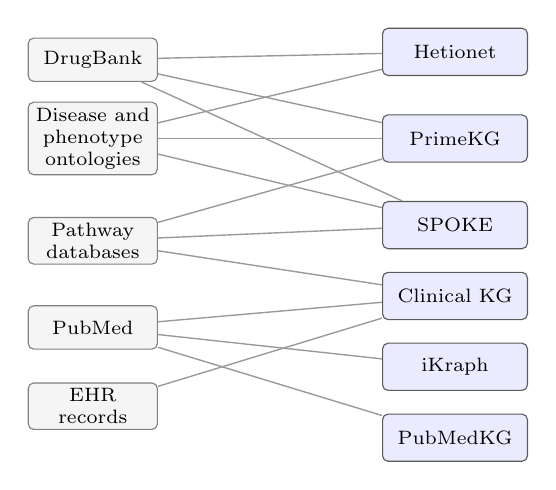
\begin{tikzpicture}[
  font=\scriptsize,
  src/.style={draw=black!50, rounded corners=2pt, fill=black!4,
              align=center, inner sep=2pt, text width=15mm, minimum height=5.5mm},
  kg/.style={draw=black!65, rounded corners=2pt, fill=blue!8,
             align=center, inner sep=2pt, text width=17mm, minimum height=6mm},
  e/.style={draw=black!40, line width=0.5pt}
]

% upstream sources
\node[src] (drugbank) at (0,0)      {DrugBank};
\node[src] (diseaseont) at (0,-1.0) {Disease and phenotype ontologies};
\node[src] (pathway) at (0,-2.3)    {Pathway databases};
\node[src] (pubmed) at (0,-3.4)     {PubMed};
\node[src] (ehr) at (0,-4.4)        {EHR records};

% derived graphs
\node[kg] (hetio) at (4.6,0.1)   {Hetionet};
\node[kg] (primekg) at (4.6,-1.0) {PrimeKG};
\node[kg] (spoke) at (4.6,-2.1)  {SPOKE};
\node[kg] (ckg) at (4.6,-3.0)    {Clinical KG};
\node[kg] (ikraph) at (4.6,-3.9) {iKraph};
\node[kg] (pkg) at (4.6,-4.8)    {PubMedKG};

% edges: shared provenance
\draw[e] (drugbank) -- (hetio);
\draw[e] (drugbank) -- (primekg);
\draw[e] (drugbank) -- (spoke);
\draw[e] (diseaseont) -- (hetio);
\draw[e] (diseaseont) -- (primekg);
\draw[e] (diseaseont) -- (spoke);
\draw[e] (pathway) -- (spoke);
\draw[e] (pathway) -- (ckg);
\draw[e] (pathway) -- (primekg);
\draw[e] (pubmed) -- (ikraph);
\draw[e] (pubmed) -- (pkg);
\draw[e] (pubmed) -- (ckg);
\draw[e] (ehr) -- (ckg);

\end{tikzpicture}%
}
\caption{Shared provenance among the representative graphs. Because several draw on the same upstream databases, two evaluations that use different graphs are not necessarily independent: an error or bias in DrugBank or in a disease ontology propagates into Hetionet, PrimeKG, and SPOKE alike. A result replicated across graphs that share sources is weaker evidence than the count of graphs suggests.}
\label{fig:provenance}
\end{figure}
